\documentclass[tikz,border=6pt]{standalone}
\usepackage{pgfplots}
\usepackage{amsmath}
\usetikzlibrary{
  arrows.meta,
  backgrounds,
  calc,
  fit,
  matrix,
  positioning,
  shapes.callouts,
  shapes.geometric,
  shapes.misc
}
\pgfplotsset{compat=1.18}

\definecolor{archInk}{HTML}{1F2933}
\definecolor{archBlue}{HTML}{0B4F6C}
\definecolor{archTeal}{HTML}{1B998B}
\definecolor{archGold}{HTML}{D98E04}
\definecolor{archRose}{HTML}{C44536}
\definecolor{archSage}{HTML}{7A9E7E}
\definecolor{archMist}{HTML}{E9F1F7}
\definecolor{archSand}{HTML}{F4F1DE}
\definecolor{archSlate}{HTML}{5C677D}
\definecolor{archStone}{HTML}{C8D0D9}

\tikzset{
  every node/.style={font=\sffamily\small, text=archInk},
  axis label/.style={font=\sffamily\footnotesize, text=archInk},
  panel/.style={
    rounded corners=6pt,
    draw=archSlate,
    line width=0.9pt,
    fill=white
  },
  stage/.style={
    panel,
    fill=archMist,
    minimum height=1.5cm,
    inner sep=7pt,
    align=left
  },
  note/.style={
    panel,
    fill=archSand,
    inner sep=7pt,
    align=left
  },
  verdict/.style={
    panel,
    fill=archTeal!12,
    inner sep=7pt,
    align=left
  },
  kill/.style={
    panel,
    fill=archRose!12,
    draw=archRose,
    inner sep=7pt,
    align=left
  },
  muted/.style={
    panel,
    fill=archStone!20,
    draw=archStone!80!archInk,
    inner sep=6pt,
    align=left
  },
  link/.style={
    -{Latex[length=3mm,width=1.7mm]},
    line width=1.0pt,
    draw=archBlue
  },
  dashedlink/.style={
    -{Latex[length=3mm,width=1.7mm]},
    line width=1.0pt,
    draw=archRose,
    dashed
  }
}

\pgfplotsset{
  every axis/.append style={
    line width=0.9pt,
    tick style={draw=archSlate},
    axis line style={draw=archSlate},
    label style={font=\sffamily\small, text=archInk},
    ticklabel style={font=\sffamily\footnotesize, text=archInk},
    legend style={
      draw=none,
      fill=white,
      font=\sffamily\footnotesize,
      text=archInk
    },
    title style={font=\sffamily\small\bfseries, text=archInk},
    grid style={draw=archStone},
    major grid style={draw=archStone},
    minor grid style={draw=archStone!70}
  }
}

\begin{document}
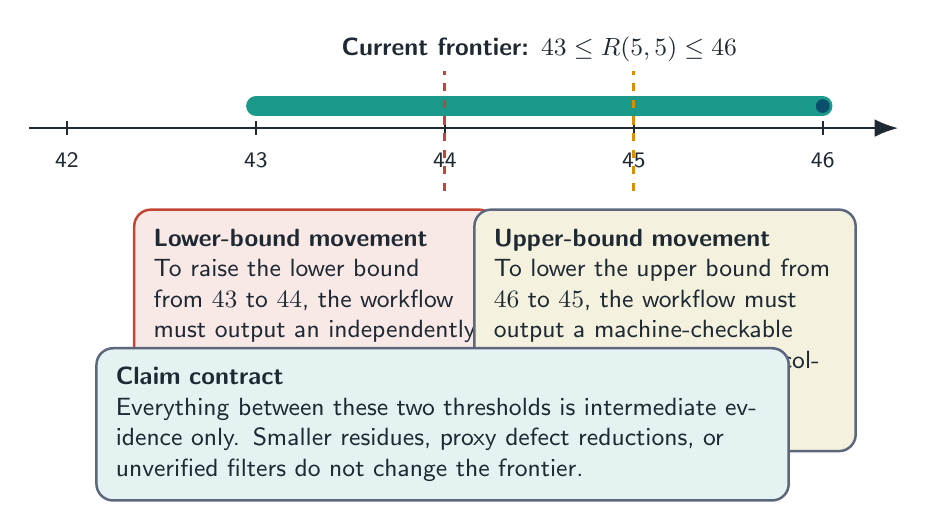
\begin{tikzpicture}[x=2.4cm,y=1cm]
  \draw[archInk, line width=1pt, -{Latex[length=3mm]}] (-0.2,0) -- (4.4,0);
  \foreach \x/\lab in {0/42,1/43,2/44,3/45,4/46} {
    \draw[archInk, line width=0.9pt] (\x,-0.09) -- (\x,0.09);
    \node[axis label, below=3pt] at (\x,-0.09) {\lab};
  }

  \draw[archTeal, line width=7pt, line cap=round] (1,0.28) -- (4,0.28);
  \fill[archTeal] (1,0.28) circle (2.5pt);
  \fill[archBlue] (4,0.28) circle (2.5pt);
  \node[font=\sffamily\bfseries\small, text=archInk] at (2.5,1.00)
    {Current frontier: $43 \le R(5,5) \le 46$};

  \draw[archRose, dashed, line width=1pt] (2,-0.8) -- (2,0.72);
  \draw[archGold, dashed, line width=1pt] (3,-0.8) -- (3,0.72);

  \node[kill, text width=4.1cm, anchor=north west] at (0.35,-1.02) {
    \textbf{Lower-bound movement}\\
    To raise the lower bound from $43$ to $44$, the workflow must output an independently
    verified $44$-vertex two-coloring with no monochromatic $K_5$.
  };

  \node[note, text width=4.35cm, anchor=north west] at (2.15,-1.02) {
    \textbf{Upper-bound movement}\\
    To lower the upper bound from $46$ to $45$, the workflow must output a machine-checkable
    proof that every $45$-vertex coloring contains a monochromatic $K_5$.
  };

  \node[verdict, text width=8.3cm, anchor=north west] at (0.15,-2.78) {
    \textbf{Claim contract}\\
    Everything between these two thresholds is intermediate evidence only. Smaller residues,
    proxy defect reductions, or unverified filters do not change the frontier.
  };
\end{tikzpicture}
\end{document}
